%%%%%%%%%%%%%%%%%%%%%%%%%%%%%%%%%%%%%%%%%
% Beamer Presentation
% LaTeX Template
% Version 1.0 (10/11/12)
%
% This template has been downloaded from:
% http://www.LaTeXTemplates.com
%
% License:
% CC BY-NC-SA 3.0 (http://creativecommons.org/licenses/by-nc-sa/3.0/)
%
%%%%%%%%%%%%%%%%%%%%%%%%%%%%%%%%%%%%%%%%%

%----------------------------------------------------------------------------------------
%	PACKAGES AND THEMES
%----------------------------------------------------------------------------------------

\documentclass{beamer}

\mode<presentation> {

% The Beamer class comes with a number of default slide themes
% which change the colors and layouts of slides. Below this is a list
% of all the themes, uncomment each in turn to see what they look like.

%\usetheme{default}
%\usetheme{AnnArbor}
%\usetheme{Antibes}
%\usetheme{Bergen}
%\usetheme{Berkeley}
%\usetheme{Berlin}
%\usetheme{Boadilla}
%\usetheme{CambridgeUS}
%\usetheme{Copenhagen}
%\usetheme{Darmstadt}
%\usetheme{Dresden}
\usetheme{Frankfurt}
%\usetheme{Goettingen}
%\usetheme{Hannover}
%\usetheme{Ilmenau}
%\usetheme{JuanLesPins}
%\usetheme{Luebeck}
%\usetheme{Madrid}
%\usetheme{Malmoe}
%\usetheme{Marburg}
%\usetheme{Montpellier}
%\usetheme{PaloAlto}
%\usetheme{Pittsburgh}
%\usetheme{Rochester}
%\usetheme{Singapore}
%\usetheme{Szeged}
%\usetheme{Warsaw}

% As well as themes, the Beamer class has a number of color themes
% for any slide theme. Uncomment each of these in turn to see how it
% changes the colors of your current slide theme.

%\usecolortheme{albatross}
%\usecolortheme{beaver}
%\usecolortheme{beetle}
%\usecolortheme{crane}
%\usecolortheme{dolphin}
%\usecolortheme{dove}
%\usecolortheme{fly}
%\usecolortheme{lily}
%\usecolortheme{orchid}
%\usecolortheme{rose}
%\usecolortheme{seagull}
%\usecolortheme{seahorse}
%\usecolortheme{whale}
%\usecolortheme{wolverine}

%\setbeamertemplate{footline} % To remove the footer line in all slides uncomment this line
%\setbeamertemplate{footline}[page number] % To replace the footer line in all slides with a simple slide count uncomment this line

%\setbeamertemplate{navigation symbols}{} % To remove the navigation symbols from the bottom of all slides uncomment this line
}

\usepackage{graphicx} % Allows including images
\usepackage{booktabs} % Allows the use of \toprule, \midrule and \bottomrule in tables
\usepackage[brazilian]{babel}
\usepackage[utf8]{inputenc}
\usepackage[T1]{fontenc}
\usepackage{amsmath}
\usepackage{animate}
\usepackage{amsmath}
\DeclareMathOperator{\atantwo}{atan2}
\newcommand{\angstrom}{\textup{\AA}}

%----------------------------------------------------------------------------------------
%	TITLE PAGE
%----------------------------------------------------------------------------------------

\title[T2]{Trabalho III} % The short title appears at the bottom of every slide, the full title is only on the title page

\author{Bruno Iochins Grisci} % Your name
\institute[UFRGS] % Your institution as it will appear on the bottom of every slide, may be shorthand to save space
{
Universidade Federal do Rio Grande do Sul \\ % Your institution for the title page
\medskip
\textit{bigrisci@inf.ufrgs.br} % Your email address
}
\date{\today} % Date, can be changed to a custom date

\begin{document}

\begin{frame}
\titlepage % Print the title page as the first slide
\end{frame}

\begin{frame}
\frametitle{Sumário} % Table of contents slide, comment this block out to remove it
\tableofcontents % Throughout your presentation, if you choose to use \section{} and \subsection{} commands, these will automatically be printed on this slide as an overview of your presentation
\end{frame}

%----------------------------------------------------------------------------------------
%	PRESENTATION SLIDES
%----------------------------------------------------------------------------------------

\section{Prelúdio}

\begin{frame}
\frametitle{Antes de começar...}
Correção da formatação do arquivo PDB do trabalho II.
\begin{figure}
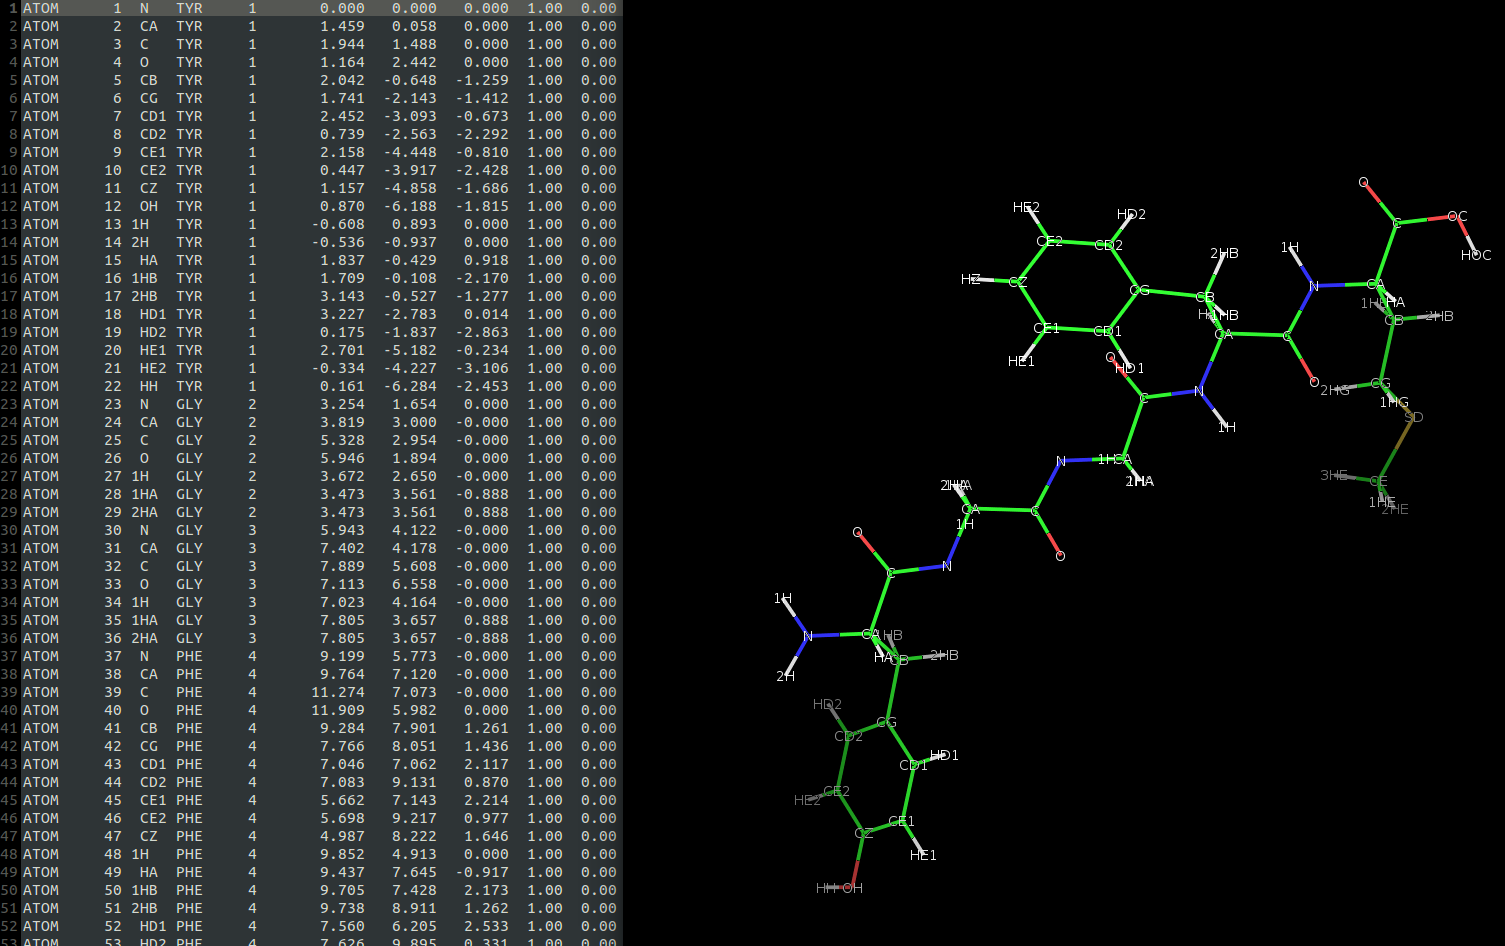
\includegraphics[width=0.9\linewidth]{1PLX-P.png}
\end{figure}
\end{frame}

\begin{frame}
\frametitle{Otimização}
Particle Swarm Optimization
\begin{itemize}
  \item Minimização
  \item Função de avaliação: $RMSD_{all}$
  \item Dimensões: $2 \times \parallel AA \parallel - 2$
  \item Limites: $[-\pi, \pi]$
  \item População: $200$
  \item Iterações: $300$
\end{itemize}
\end{frame}

\begin{frame}
\frametitle{Minimização do RMSD}
\begin{figure}
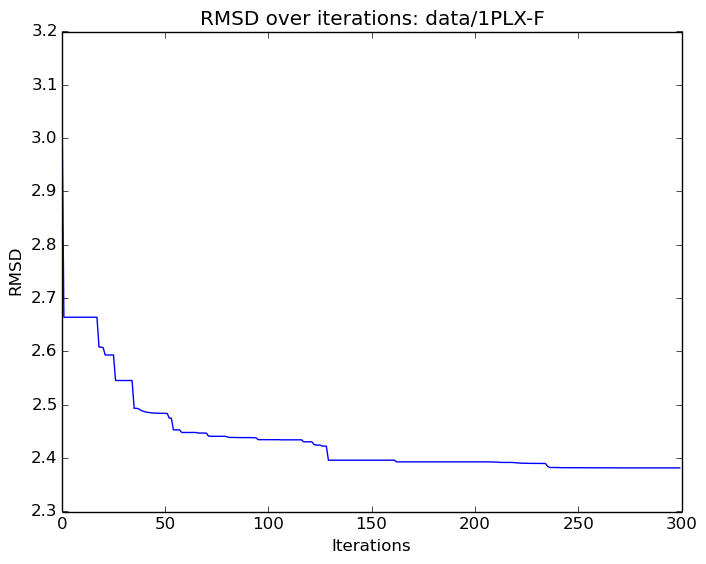
\includegraphics[width=0.7\linewidth]{1PLX-F_rmsd.png}
\end{figure}
Tempo de execução: $19$ minutos
\end{frame}

\begin{frame}
\frametitle{Resultados}
\begin{itemize}
  \item $RMSD_{C_\alpha}: 0.40 \angstrom$
  \item $RMSD_{backbone}: 0.83 \angstrom$
  \item $RMSD_{all}: 2.38 \angstrom$ 
\end{itemize}
\begin{figure}
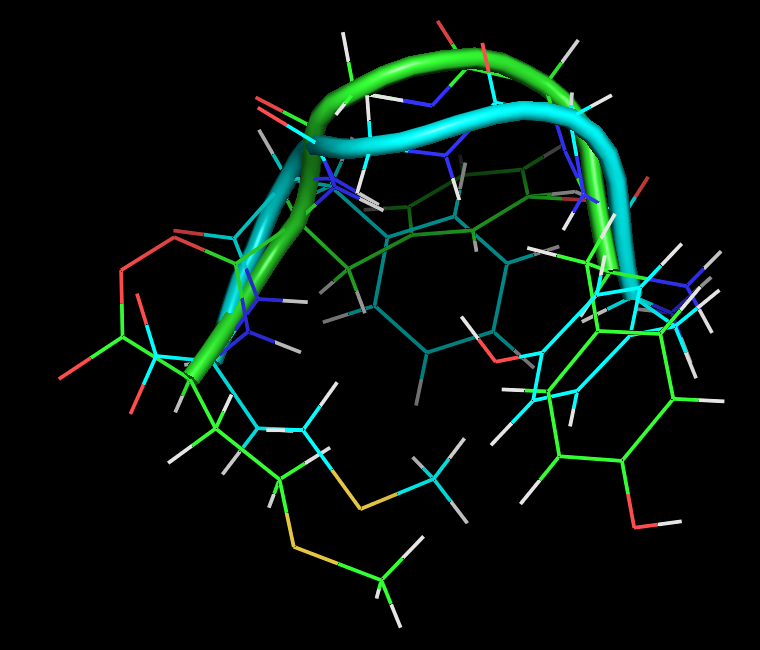
\includegraphics[width=0.5\linewidth]{1PLX-F.png}
\end{figure}
\end{frame}

\begin{frame}
\frametitle{Ângulos (1PLX x 1PLX-F)}
\begin{table}[]
\centering
\label{my-label}
\begin{tabular}{llll}
AA & PHI             &  PSI              &  OMEGA             \\
TYR         & 360.00 x 360.00 &  176.63 x -115.80 &  360.00 x  360.00  \\
GLY         & 148.48 x 121.15 &  -21.96 x   10.17 &  179.86 x  179.98  \\
GLY         & 114.02 x  78.37 &   29.89 x   35.39 &  179.81 x -179.99  \\
PHE         & -88.00 x -81.96 &  -38.16 x  -93.28 &  179.75 x  179.97  \\
MET         & -74.24 x  -9.66 &  360.00 x  360.00 & -179.95 x  180.00
\end{tabular}
\end{table}
\end{frame}

%------------------------------------------------
\section{Criação da proteína} % Sections can be created in order to organize your presentation into discrete blocks, all sections and subsections are automatically printed in the table of contents as an overview of the talk

\begin{frame}
\frametitle{Ferramentas}
\begin{itemize}
\item Python;
\item Numpy;
\item Orientado a Objetos;
\item Trabalhos I e II.
\end{itemize}
\end{frame}

\begin{frame}
\frametitle{1L2Y}
\begin{itemize}
\item Sequência: NLYIQWLKDGGPSSGRPPPS;
\item 1L2Y x 1L2Y-P:
\begin{itemize}
  \item $RMSD_{C_\alpha}: 17.89 \angstrom$
  \item $RMSD_{backbone}: 18.08 \angstrom$
  \item $RMSD_{all}: 19.13 \angstrom$ 
\end{itemize}
\end{itemize}
\begin{figure}
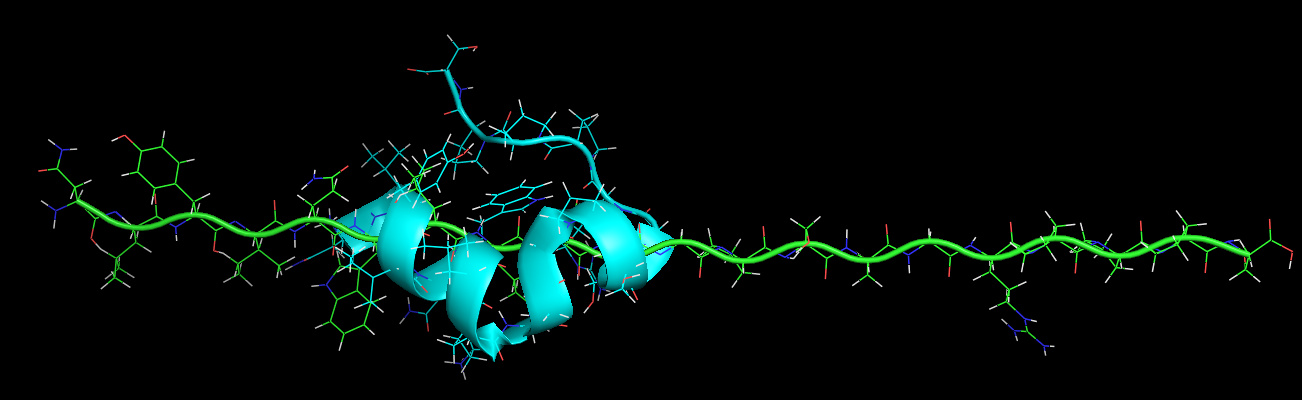
\includegraphics[width=0.7\linewidth]{1L2Y.png}
\end{figure}
\end{frame}

%------------------------------------------------
\section{Implementação} % Sections can be created in order to organize your presentation into discrete blocks, all sections and subsections are automatically printed in the table of contents as an overview of the talk
%------------------------------------------------

\begin{frame}
\frametitle{Energia Potencial (AMBER99)}
$E_{total} = $

$\sum_{bonds} K_{b}(b - b_0)^2 + $

$\sum_{UB} K_{UB}(S - S_0)^2 + $

$\sum_{angle} K_{\theta}(\theta - \theta_0)^2 + $

$\sum_{dihedrals} K_{\chi}(1 + cos(\eta - \delta)) + $

$\sum_{impropers} K_{imp}(\varphi - \varphi_0)^2 + $

$\color{red}\sum_{nonbond} \varepsilon_{ij} [(\frac{R_{minij}}{r_{ij}})^{12} -2(\frac{R_{minij}}{r_{ij}})^6] + \varepsilon_1 \frac{q_i q_j}{r_{ij}} $
\end{frame}

\begin{frame}
\frametitle{Termos não ligados}
$\varepsilon_{ij} = \sqrt{ \color{red} \varepsilon_i \varepsilon_j \color{black} }$

$R_{mini} = \color{red}\sigma_i \color{black} \cdot 2^{1/6}$

$r_{ij} = \parallel P_i - P_j \parallel \color{blue}/10 (nm) \color{black}$ 

$R_{minij} = \frac{R_{mini} + R_{minj}}{2}$

$U^{LJ}_{ij} = \sqrt{ \color{red} \varepsilon_i \varepsilon_j \color{black} } [(\frac{R_{mini} + R_{minj}}{2r_{ij}})^{12} -2(\frac{R_{mini} + R_{minj}}{2r_{ij}})^{6}]$

$\varepsilon_1 = 9 \cdot 10^9 \color{blue} \cdot \frac{(1.6022 \cdot 10^{-19})^2}{1 \cdot 10^{-9}} \cdot \frac{6.022140857 \cdot 10^{23}}{1000} (kJ/mol) \color{black}$

$E_{nonbond} = \sum_{nonbond} \varepsilon_{ij} [(\frac{R_{minij}}{r_{ij}})^{12} -2(\frac{R_{minij}}{r_{ij}})^6] + \varepsilon_1 \frac{\color{red}q_i q_j \color{black}}{r_{ij}}$
\end{frame}

\begin{frame}
\frametitle{Otimização}
Particle Swarm Optimization
\begin{itemize}
  \item Minimização;
  \item Função de avaliação: $E_{nonbond}$ (AMBER99);
  \item Dimensões: $2 \times \parallel AA \parallel - 2$;
  \item Limites: $[-\pi, \pi]$;
  \item População: $60$;
  \item Iterações: $200$
\end{itemize}
\end{frame}

%------------------------------------------------
\section{Resultados} % Sections can be created in order to organize your presentation into discrete blocks, all sections and subsections are automatically printed in the table of contents as an overview of the talk
%------------------------------------------------

\begin{frame}
\frametitle{Energia X RMSD}
\begin{figure}
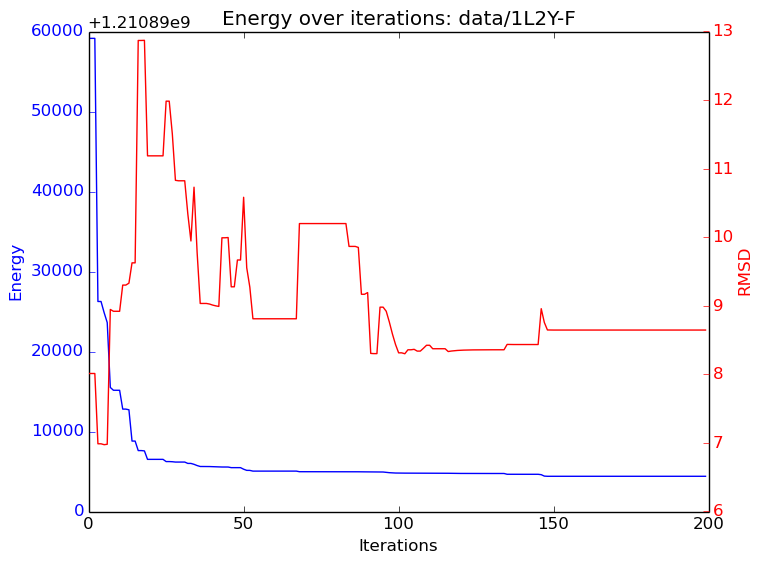
\includegraphics[width=0.7\linewidth]{1L2Y-F200_energy.png}
\end{figure}
Tempo: 3h 48 min
\end{frame}

\begin{frame}
\frametitle{Energias}
\begin{itemize}
  \item $E_{nonbond}^{1L2Y}: 35,576.37 kJ/mol$
  \item $E_{nonbond}^{1L2Y-P}: 1,211,016,661.41 kJ/mol$
  \item $E_{nonbond}^{1L2Y-F}: 1,210,894,401.45 kJ/mol$
\end{itemize} 
\end{frame}

\begin{frame}
\frametitle{1L2Y X 1L2Y-F}
\begin{figure}
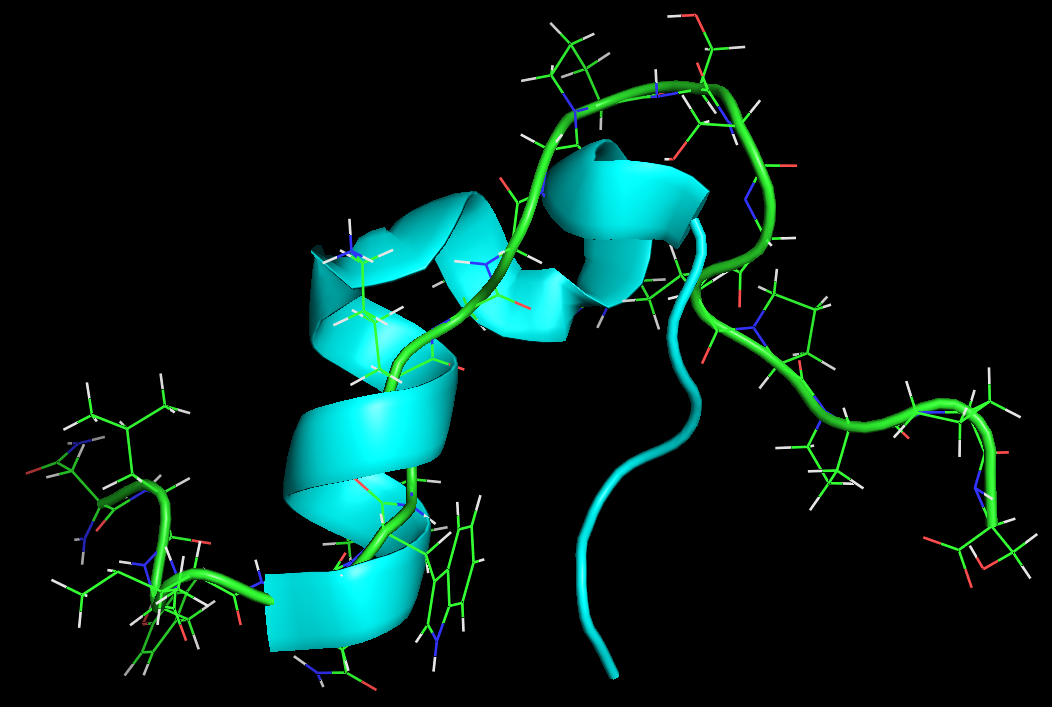
\includegraphics[width=0.6\linewidth]{1L2Y-F.png}
\end{figure}
\begin{itemize}
  \item $RMSD_{C_\alpha}: 6.83\angstrom$
  \item $RMSD_{backbone}: 6.74\angstrom$
  \item $RMSD_{all}: 8.64\angstrom$ 
\end{itemize}
\end{frame}

\begin{frame}
\Huge{\centerline{Fim}}
\end{frame}

%----------------------------------------------------------------------------------------

\end{document} 